%==============================================================================
% presentation.tex
%==============================================================================


%==============================================================================
% Configuration
%==============================================================================

% Internationalisation
\usepackage[utf8]{inputenc}
\usepackage[T1]{fontenc}
% \usepackage[ngerman]{babel}

% Different packages
\usepackage{url}
\usepackage{color,listings,paralist}
\usepackage{enumerate}
\usepackage{tabularx}
\usepackage{alltt}

% Use default Acrobat reader fonts
\usepackage{mathpazo}

% Use CM fonts (increases document size)
\usepackage{ae}

% Use images
\usepackage{graphicx}

% Configure beamer
\usetheme[secheader]{Ikhono}
\usefonttheme[onlylarge]{structurebold}
\setbeamertemplate{navigation symbols}{}

% Variables
\providecommand{\Title}{Parallel Programming}
\providecommand{\Subtitle}{Recitation Session 2}
\providecommand{\Author}{Thomas Weibel <weibelt@ethz.ch>}
\providecommand{\Institute}{Laboratory for Software Technology, \\
  Swiss Federal Institute of Technology Z\"urich}
\providecommand{\Date}{March 10, 2010}

% PDF settings
\hypersetup{
  pdftitle={\Title, \Subtitle},
  pdfauthor={\Author},
  pdfsubject={\Institute},
  pdfkeywords={parallel programming} 
}

% Titlepage
\title{\Title}
\subtitle{\Subtitle}
\author{\Author}
\institute{\Institute}
\date{\Date}

% Listings
\lstdefinestyle{Default}{
  language=Java,
  tabsize=2,
  mathescape=true,
  inputencoding=utf8,
  showstringspaces=false,
  fontadjust=true,
  basicstyle=\ttfamily,
  keywordstyle=\color{blue}\bfseries,
}
\lstset{style=Default}


%==============================================================================
% Document
%==============================================================================

\begin{document}


% Titlepage
\begin{frame}[plain]
  \titlepage
\end{frame}


\section*{Introduction}

\begin{frame}{Executive Summary}
  \begin{itemize}
  \item Solution to the last assignment
  \item Threads in Java
    \begin{itemize}
    \item Create and start
    \item Synchronization
    \item Deadlocks
    \end{itemize}
  \item Producer/Consumer
  \item Hints for the next assignment
  \end{itemize}
\end{frame}


\section{Last Assignment}

\begin{frame}{Outline}
  \tableofcontents[current]
\end{frame}

\begin{frame}[fragile]{Solution}
  \begin{lstlisting}[basicstyle=\ttfamily\small]
class Incrementer {
  public static void process(String arg) 
      throws TerminationException {
    int tmp = Integer.parseInt(arg);
    if (tmp < 0)
      throw(new TerminationException("< 0"));
    System.out.println(tmp+1);    
  }  
  public static void main(String[] args) {
    try {
      for (int i = 0; i < args.length; i++)
        process(args[i]);
    }
    catch (TerminationException e) {
      System.out.println(e.getMessage()); 
    } 
  }
} 
  \end{lstlisting}
\end{frame}

\begin{frame}{Formatting Source Code}
  \begin{itemize}
  \item 80\% of the lifetime cost of a software product goes to
    maintenance
  \item Hardly any software is maintained for its whole life by the
    original author(s)
  \item Using good style improves the maintainability of software
    code
  \item Eclipse: ``Ctrl+Shift+F'' or ``Source $\rightarrow$ Format''
  \end{itemize}

  \vspace{\stretch{1}}

  \begin{center}
    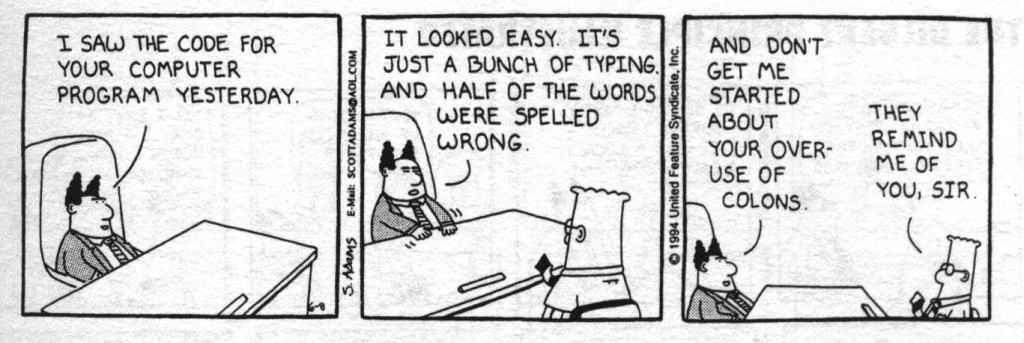
\includegraphics[scale=0.3]{figures/dilbert-1}
  \end{center}
\end{frame}

\begin{frame}[fragile]{Java Naming Conventions}
  \begin{itemize}
  \item Non-static variables and methods use camel case:
    \begin{itemize}
    \item \lstinline!thisIsAVariable!
    \item \alert{not} \lstinline!this_is_a_variable!
    \end{itemize}
  \item Class and interface names should start with capital:
    \begin{itemize}
    \item \lstinline!LinkedList!
    \item \alert{not} \lstinline!LINKED_LIST!
    \end{itemize}
  \item Non-static variable and all function names should start with
    lower case: \lstinline!readFromFile()! or \lstinline!firstName!
  \item All static variables upper-case: \lstinline!MAXIMUM_USERS!
  \item Package names should be all lowercase, with no spaces between
    words: \lstinline!ch.ethz.inf!
  \end{itemize}
\end{frame}

\begin{frame}[fragile]{Pre and Post Increment}
  Pre Increment:

  \vspace{\stretch{1}}

  \begin{lstlisting}
  int i = 41;
  System.out.println(++i);
  System.out.println(i);
  \end{lstlisting}

  \vspace{\stretch{1}}

  Post Increment:

  \vspace{\stretch{1}}

  \begin{lstlisting}
  int j = 23;
  System.out.println(j++);
  System.out.println(j);
  \end{lstlisting}

  \vspace{\stretch{1}}

  Output?
\end{frame}

\begin{frame}[fragile]{Conditional Operator (Ternary Operator)}
  \begin{lstlisting}
  if (a > b) {
    max = a;
  }
  else {
    max = b;
  }    
  \end{lstlisting}

  \vspace{\stretch{1}}

  can be written with the conditional operator \lstinline!?:! as

  \vspace{\stretch{1}}

  \begin{lstlisting}
  max = (a > b) ? a : b;
  \end{lstlisting}

  \vspace{\stretch{1}}

  Use it wisely!
\end{frame}


\section{Threads}

\begin{frame}{Outline}
  \tableofcontents[current]
\end{frame}

\begin{frame}{Creating Threads}
  An application that creates an instance of \lstinline!Thread! must
  provide the code that will run in that thread. There are two ways to
  do this:

  \vspace{\stretch{1}}

  \begin{itemize}
  \item Provide a \lstinline!Runnable! object
  \item Subclass \lstinline!Thread!
  \end{itemize}
\end{frame}

\begin{frame}[fragile]{Runnable Object}
  \begin{itemize}
  \item \lstinline!Runnable! interface defines a single method:
    \lstinline!run!
  \item Meant to contain the code executed in the thread
  \item The \lstinline!Runnable! object is passed to the
    \lstinline!Thread! constructor
  \end{itemize}

  \vspace{\stretch{1}}

  \begin{lstlisting}
public class HelloRunnable 
   implements Runnable {
  public void run() {
    System.out.println("Hello from a thread!");
  }
  
  public static void main(String args[]) {
    (new Thread(new HelloRunnable())).start();
  }
}
  \end{lstlisting}
\end{frame}

\begin{frame}[fragile]{Subclass Thread}
  \begin{itemize}
  \item The \lstinline!Thread! class itself implements
    \lstinline!Runnable!
  \item Its \lstinline!run! method does nothing
  \item Application can subclass \lstinline!Thread!, providing its own
    implementation of \lstinline!run!
  \end{itemize}

  \vspace{\stretch{1}}

  \begin{lstlisting}
public class HelloThread extends Thread {
  public void run() {
    System.out.println("Hello from a thread!");
  }
  
  public static void main(String args[]) {
    (new HelloThread()).start();
  }  
}
  \end{lstlisting}
\end{frame}

\begin{frame}{Threads}
  \begin{itemize}
  \item \lstinline!Runnable! object: more general, can subclass a
    class other than \lstinline!Thread!
  \item Subclass \lstinline!Thread!: easier to use in simple
    applications, but limited by the fact that task class must be a
    descendant of \lstinline!Thread!
  \item Invoke \lstinline!threadInstance.start()! to start the new
    thread
  \item \alert{Note:} \lstinline!threadInstance.run()! does not create
    a new thread
  \end{itemize}
\end{frame}

\begin{frame}[fragile]{Sleep}
  \begin{lstlisting}
  try {	
    // Doze a random time (0 to 0.5 secs)	
    // to simulate workload	
    Thread.sleep((int)(Math.random()*500));
  } 
  catch (InterruptedException e) { 
    // ... 
  }  
  \end{lstlisting}

  \vspace{\stretch{1}}

  \begin{itemize}
  \item \lstinline!Thread.sleep(long)! puts the current thread to
    sleep for the specified time in milliseconds
  \item An \lstinline!InterruptedException! is thrown when a thread is
    waiting, sleeping, or otherwise paused for a long time and another
    thread interrupts it using the \lstinline!interrupt! method in
    class \lstinline!Thread!
  \end{itemize}
\end{frame}

\begin{frame}[fragile]{Synchronized}
  \begin{itemize}
  \item Every class and every object has an intrinsic lock
  \item \lstinline!synchronized! marks code blocks where a thread must
    acquire the lock before proceeding
  \item \lstinline!synchronized! can be added to methods
  \item The \lstinline!this! pointer is used as the lock for instance
    methods
  \end{itemize}

  \vspace{\stretch{1}}

  \begin{lstlisting}
public class Buffer {
  public synchronized void write(int i) {
    // ... 
  }
  
  public synchronized int read() {
    // ... 
  }
}
  \end{lstlisting}
\end{frame}

\begin{frame}[fragile]{Synchronized}
  \begin{itemize}
  \item \lstinline{synchronized} can also be used to guard arbitrary
    blocks of code within a method, even in different classes
  \item It is important to use the correct object as the locks!
  \end{itemize}

  \vspace{\stretch{1}}

 \begin{lstlisting}
   public void someMethod1() {
     //do something before
     synchronized(anObject) { /* ... */ }
     //do something after
   }

   public void someMethod2() {
     //do something before
     synchronized(anObject) { /* ... */ }
     //do something after
   }   
 \end{lstlisting}
\end{frame}

\begin{frame}{Quiz}
  \begin{itemize}
  \item Can static methods be synchronized?
  \item What is the lock ``object''?
  \item What is a deadlock?
  \item How can a deadlock occur?
  \end{itemize}

  \vspace{\stretch{1}}

  \begin{center}
    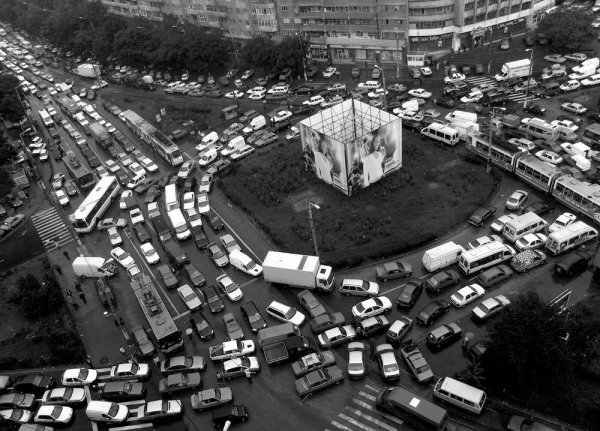
\includegraphics[scale=0.33]{figures/deadlock} \\
    \tiny{Source: \url{http://www.vijayforvictory.com}}    
  \end{center}
\end{frame}

\begin{frame}{Deadlock}
  \begin{itemize}
  \item Deadlock describes a situation where two or more threads are
    blocked forever, waiting for each other
  \item
    \url{http://java.sun.com/docs/books/tutorial/essential/concurrency/deadlock.html}:
    \begin{itemize}
    \item Alphonse and Gaston are friends, and great believers in
      courtesy
    \item A strict rule of courtesy is that when you bow to a friend,
      you must remain bowed until your friend has a chance to return
      the bow
    \item Unfortunately, this rule does not account for the
      possibility that two friends might bow to each other at the same
      time
    \item What happens if both bow at the same time?
    \end{itemize}
  \item Analyze deadlocks: ``Ctrl+\textbackslash" (Unix),
    ``Ctrl+Break'' (Windows)
  \end{itemize}
\end{frame}


\section{Producer/Consumer}

\begin{frame}{Outline}
  \tableofcontents[current]
\end{frame}

\begin{frame}{Once Upon a Time \ldots}
  \begin{center}
    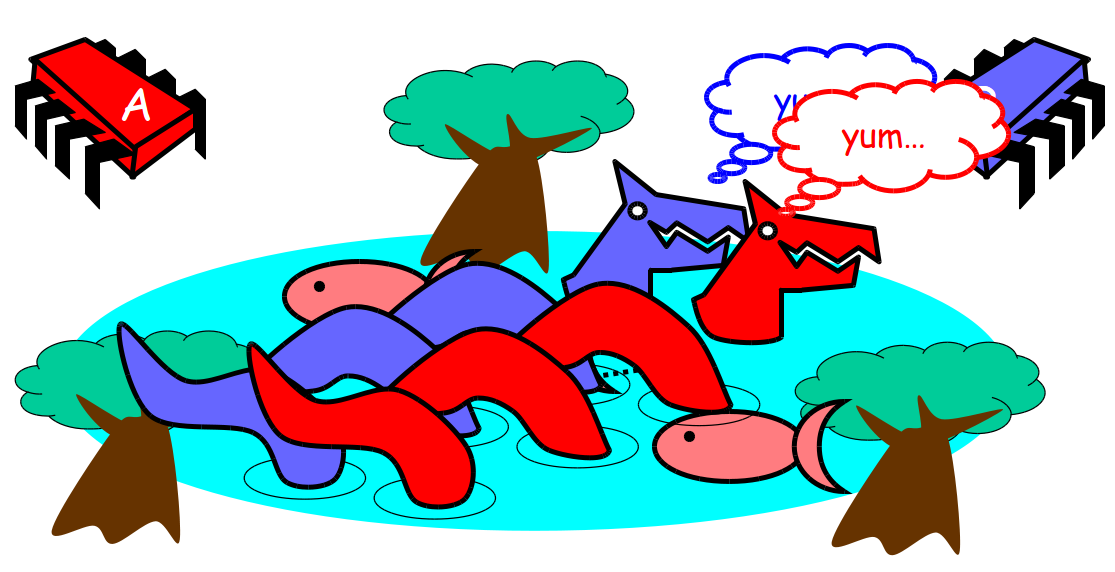
\includegraphics[scale=0.35]{figures/pets-1}
  \end{center}

  \vspace{\stretch{1}}

  \begin{itemize}
  \item Alice and Bob own a pet they bring to the same pond to feed
  \item Alice and Bob fall in love \& marry
  \item Then they fall out of love \& divorce
    \begin{itemize}
    \item She gets the pets
    \item He has to feed them
    \end{itemize}
  \end{itemize}

  \tiny{Example: ``The Art of Multiprocessor Programming'', Herlihy,
    Creative Commons Attribution-ShareAlike 2.5 License}
\end{frame}

\begin{frame}{Bob Puts Food in the Pond}
  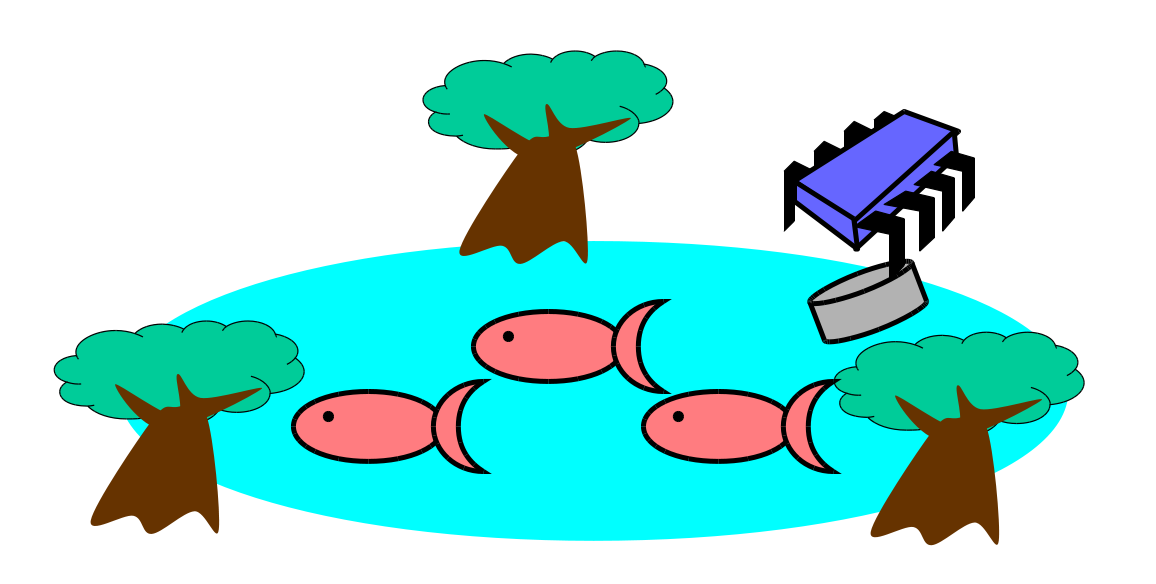
\includegraphics[width=\textwidth]{figures/pets-2}
\end{frame}

\begin{frame}{Alice Releases Her Pets to Feed}
  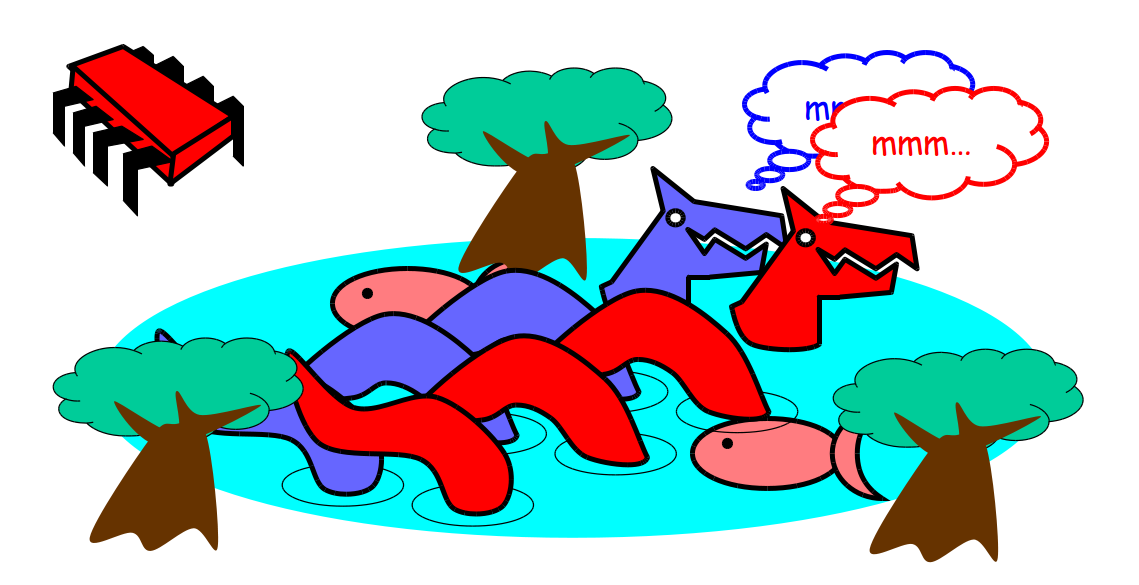
\includegraphics[width=\textwidth]{figures/pets-3}
\end{frame}

\begin{frame}{Producer/Consumer}
  \begin{itemize}
  \item   Alice and Bob can't meet
    \begin{itemize}
    \item Each has restraining order on other
    \item So he puts food in the pond
    \item And later, she releases the pets
    \end{itemize}
  \item Avoid
    \begin{itemize}
    \item Releasing pets when there's no food
    \item Putting out food if uneaten food remains
    \end{itemize}
  \end{itemize}
\end{frame}

\begin{frame}{Producer/Consumer}
  Need a mechanism so that

  \vspace{\stretch{1}}

  \begin{itemize}
  \item Bob lets Alice know when food has been put out
  \item Alice lets Bob know when to put out more food  
  \end{itemize}
\end{frame}

\begin{frame}{Solution}
  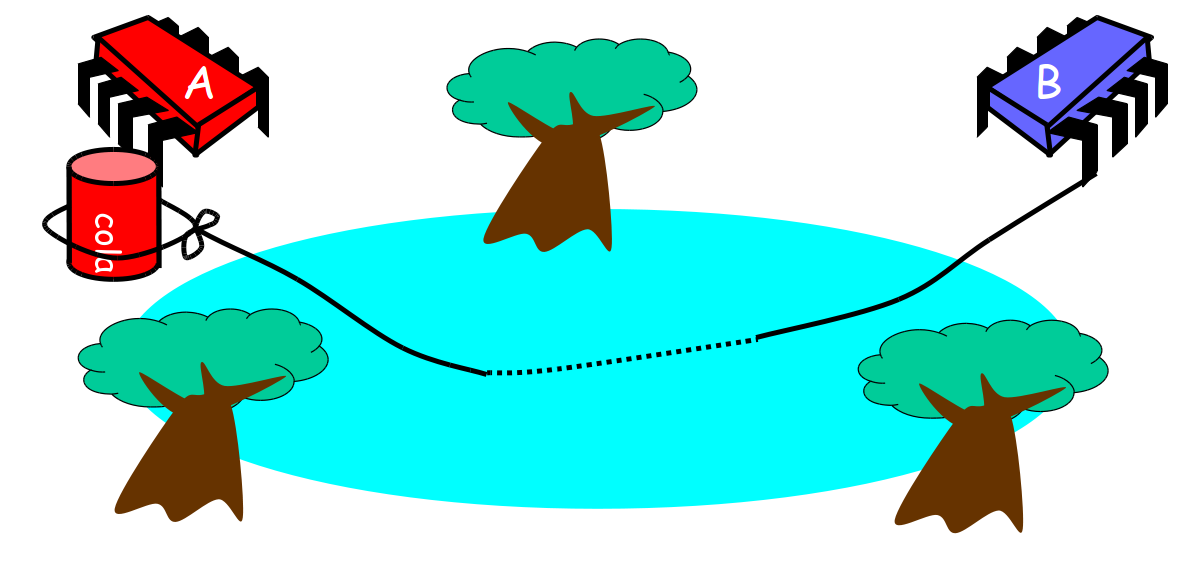
\includegraphics[width=\textwidth]{figures/pets-4}
\end{frame}

\begin{frame}{Bob puts food in Pond}
  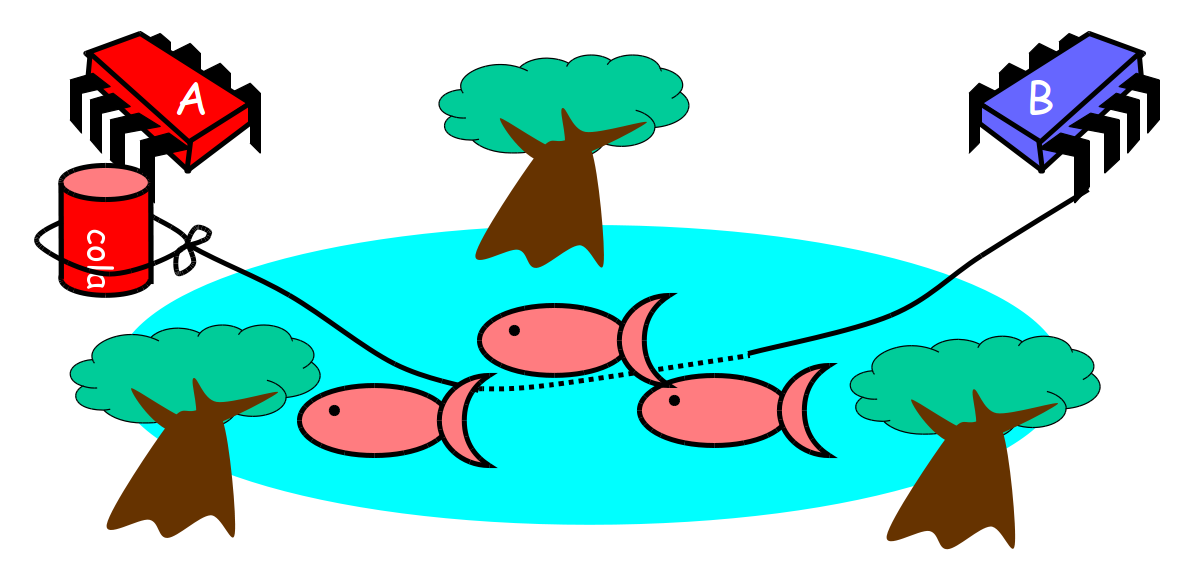
\includegraphics[width=\textwidth]{figures/pets-5}
\end{frame}

\begin{frame}{Bob knocks over Can}
  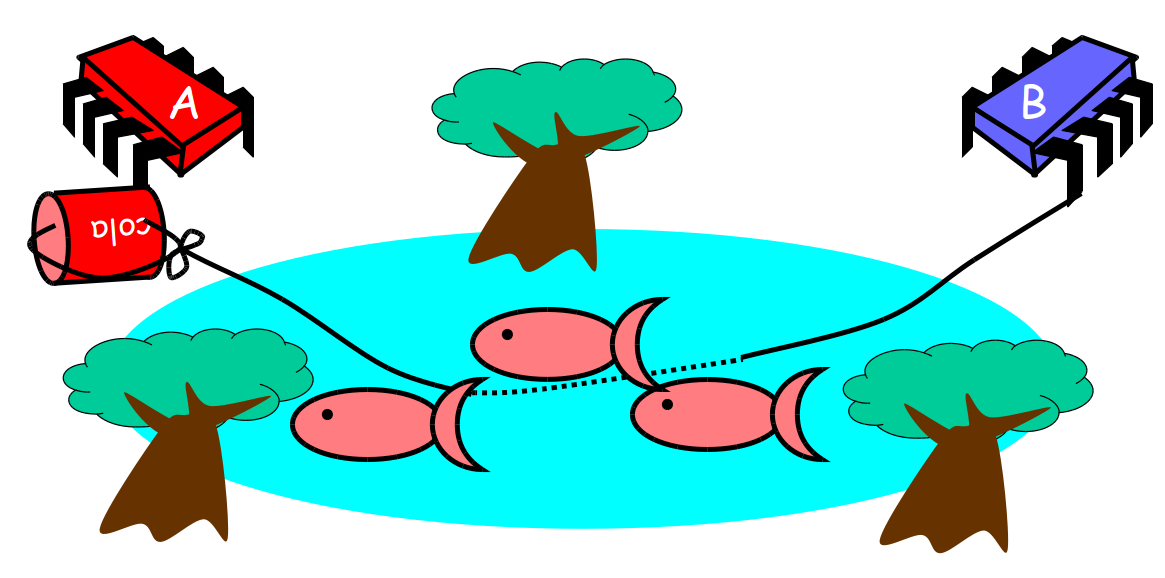
\includegraphics[width=\textwidth]{figures/pets-6}
\end{frame}

\begin{frame}{Alice Releases Pets}
  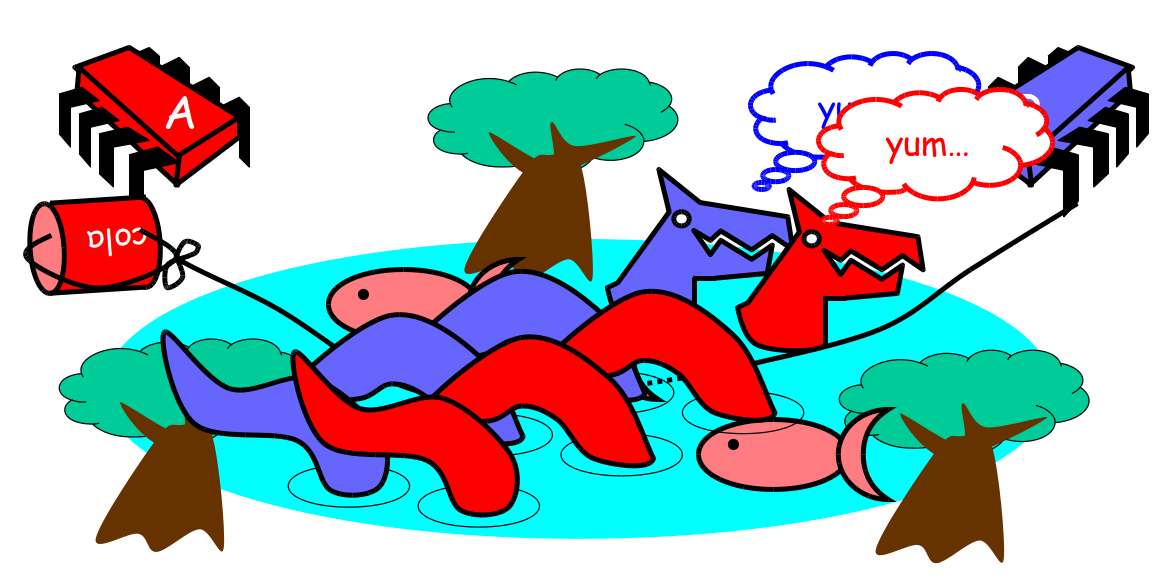
\includegraphics[width=\textwidth]{figures/pets-7}
\end{frame}

\begin{frame}{Alice Resets Can when Pets are Fed}
  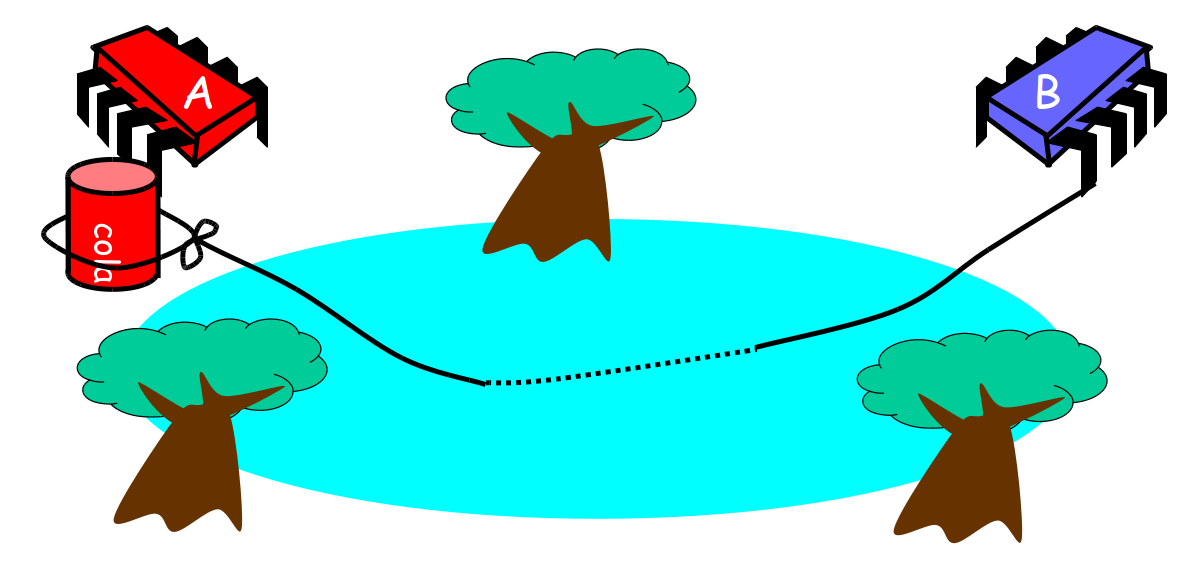
\includegraphics[width=\textwidth]{figures/pets-8}
\end{frame}

\begin{frame}[fragile]{Pseudocode}
  Alice:
  \begin{lstlisting}
  while (true) {
    while (can.isUp()){};
    pet.release();
    pet.recapture();
    can.reset();
  }
  \end{lstlisting}

  \vspace{\stretch{1}}
  
  Bob:
  \begin{lstlisting}
  while (true) {
    while (can.isDown()){};
    pond.stockWithFood();
    can.knockOver();
  } 
  \end{lstlisting}
\end{frame}

\begin{frame}{Correctness}
  \begin{itemize}
  \item Mutual Exclusion: Pets and Bob never together in pond.
  \item No Starvation: if Bob always willing to feed, and pets always
    famished, then pets eat infinitely often.
  \item Producer/Consumer: The pets never enter pond unless there is
    food, and Bob never provides food if there is unconsumed food.
  \end{itemize}
\end{frame}


\section{New Assignment}

\begin{frame}{Outline}
  \tableofcontents[current]
\end{frame}

\begin{frame}{Buffer}
  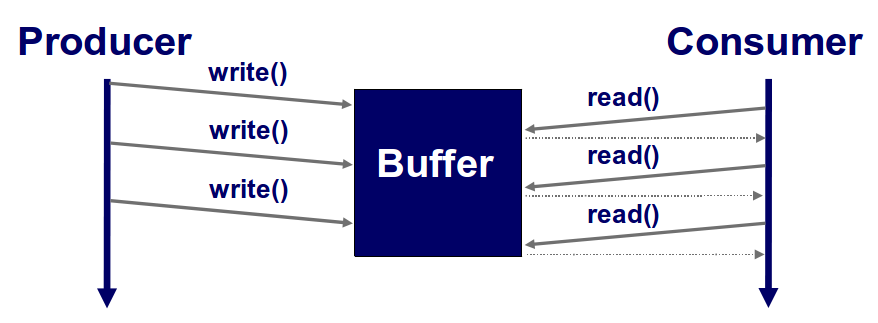
\includegraphics[width=\textwidth]{figures/buffer}

  \vspace{\stretch{1}}

  \begin{itemize}
  \item A producer thread constantly produces values and writes them
    into a shared buffer
  \item A consumer thread reads a value from the shared buffer and
    uses it
  \item Premise: Every value must be consumed exactly once
  \item Question: How to synchronize those two?
  \end{itemize}
\end{frame}


\section*{Outro}

\begin{frame}{Summary}
  \begin{itemize}
  \item Create and start threads
  \item Thread synchronization
  \item Problem with synchronization: Deadlocks
  \item Producer/Consumer pattern
  \end{itemize}

  \vspace{\stretch{1}}

  \begin{center}
    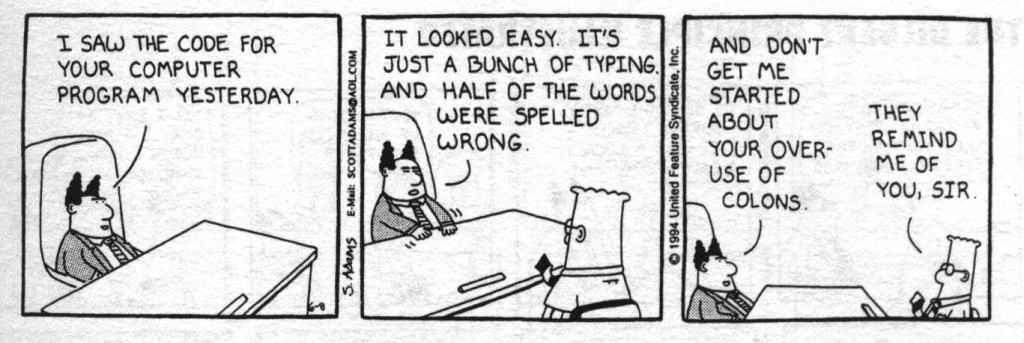
\includegraphics[width=\textwidth]{figures/dilbert-2}
  \end{center}
\end{frame}

\end{document}
